\documentclass{standalone}


% Copy of relevant parts from the main preamble.
\usepackage{mathtools}

% Uncomment the following to use Times New Roman and Cambria Math
% \usepackage{unicode-math}
% \unimathsetup{math-style=TeX}
% \setmathfont[range=\mathup/{num}]{Times New Roman}
% \setmathfont[range=\mathit/{greek,Greek,latin,Latin}]{Cambria Math}
% \setmathfont[range=\mathup/{greek,Greek,latin,Latin}]{Cambria Math}
% \setmathfont[range={"2212,"002B,"003D,"0028,"0029,"005B,"005D,"221A,
% "2211,"2248,"222B,"007C,"2026,"2202,"00D7,"0302,"2261,"0025,"22C5,
% "00B1,"2194,"21D4,"2032}]
% {Cambria Math}
% \setmainfont[Ligatures=TeX]{Times New Roman}

% Uncomment the following to use Linux Libertine
% \usepackage[libertine]{newtxmath}
% \usepackage[no-math]{fontspec}
% \setmainfont{Linux Libertine O}

% Uncomment the following to use TeX Gyre Termes
% \usepackage{unicode-math}
% \unimathsetup{math-style=TeX}
% \setmainfont{TeX Gyre Termes}
% \setmathfont{TeX Gyre Termes Math}

% Uncomment the following to use TeX Gyre Pagella
\usepackage{unicode-math}
\unimathsetup{math-style=TeX}
\setmainfont{TeX Gyre Pagella}
\setmathfont{TeX Gyre Pagella Math}

% \usepackage[sfmath]{kpfonts}
% \renewcommand*\familydefault{\sfdefault}
% \usepackage[T1]{fontenc}

% \usepackage[no-math]{fontspec}
% Always use Inconsolata
\setmonofont{Inconsolata}

\usepackage{microtype}


\usepackage[version=3]{mhchem}
\usepackage{chemfig}
\setatomsep{2.25em}
\usetikzlibrary{positioning, calc, arrows.meta}
\tikzset{
    flux/.style={
        right,
        align=left,
    },
}
\usepackage{siunitx}
\sisetup{detect-all=true}
\newcommand*{\flux}[3]{\SI{#1}{\percent}\\\textbf{\SI{#2}{\percent}}\\\textit{\SI{#3}{\percent}}}
\newcommand*{\iPeOH}{\textit{i}-Pentenol}

\begin{document}
    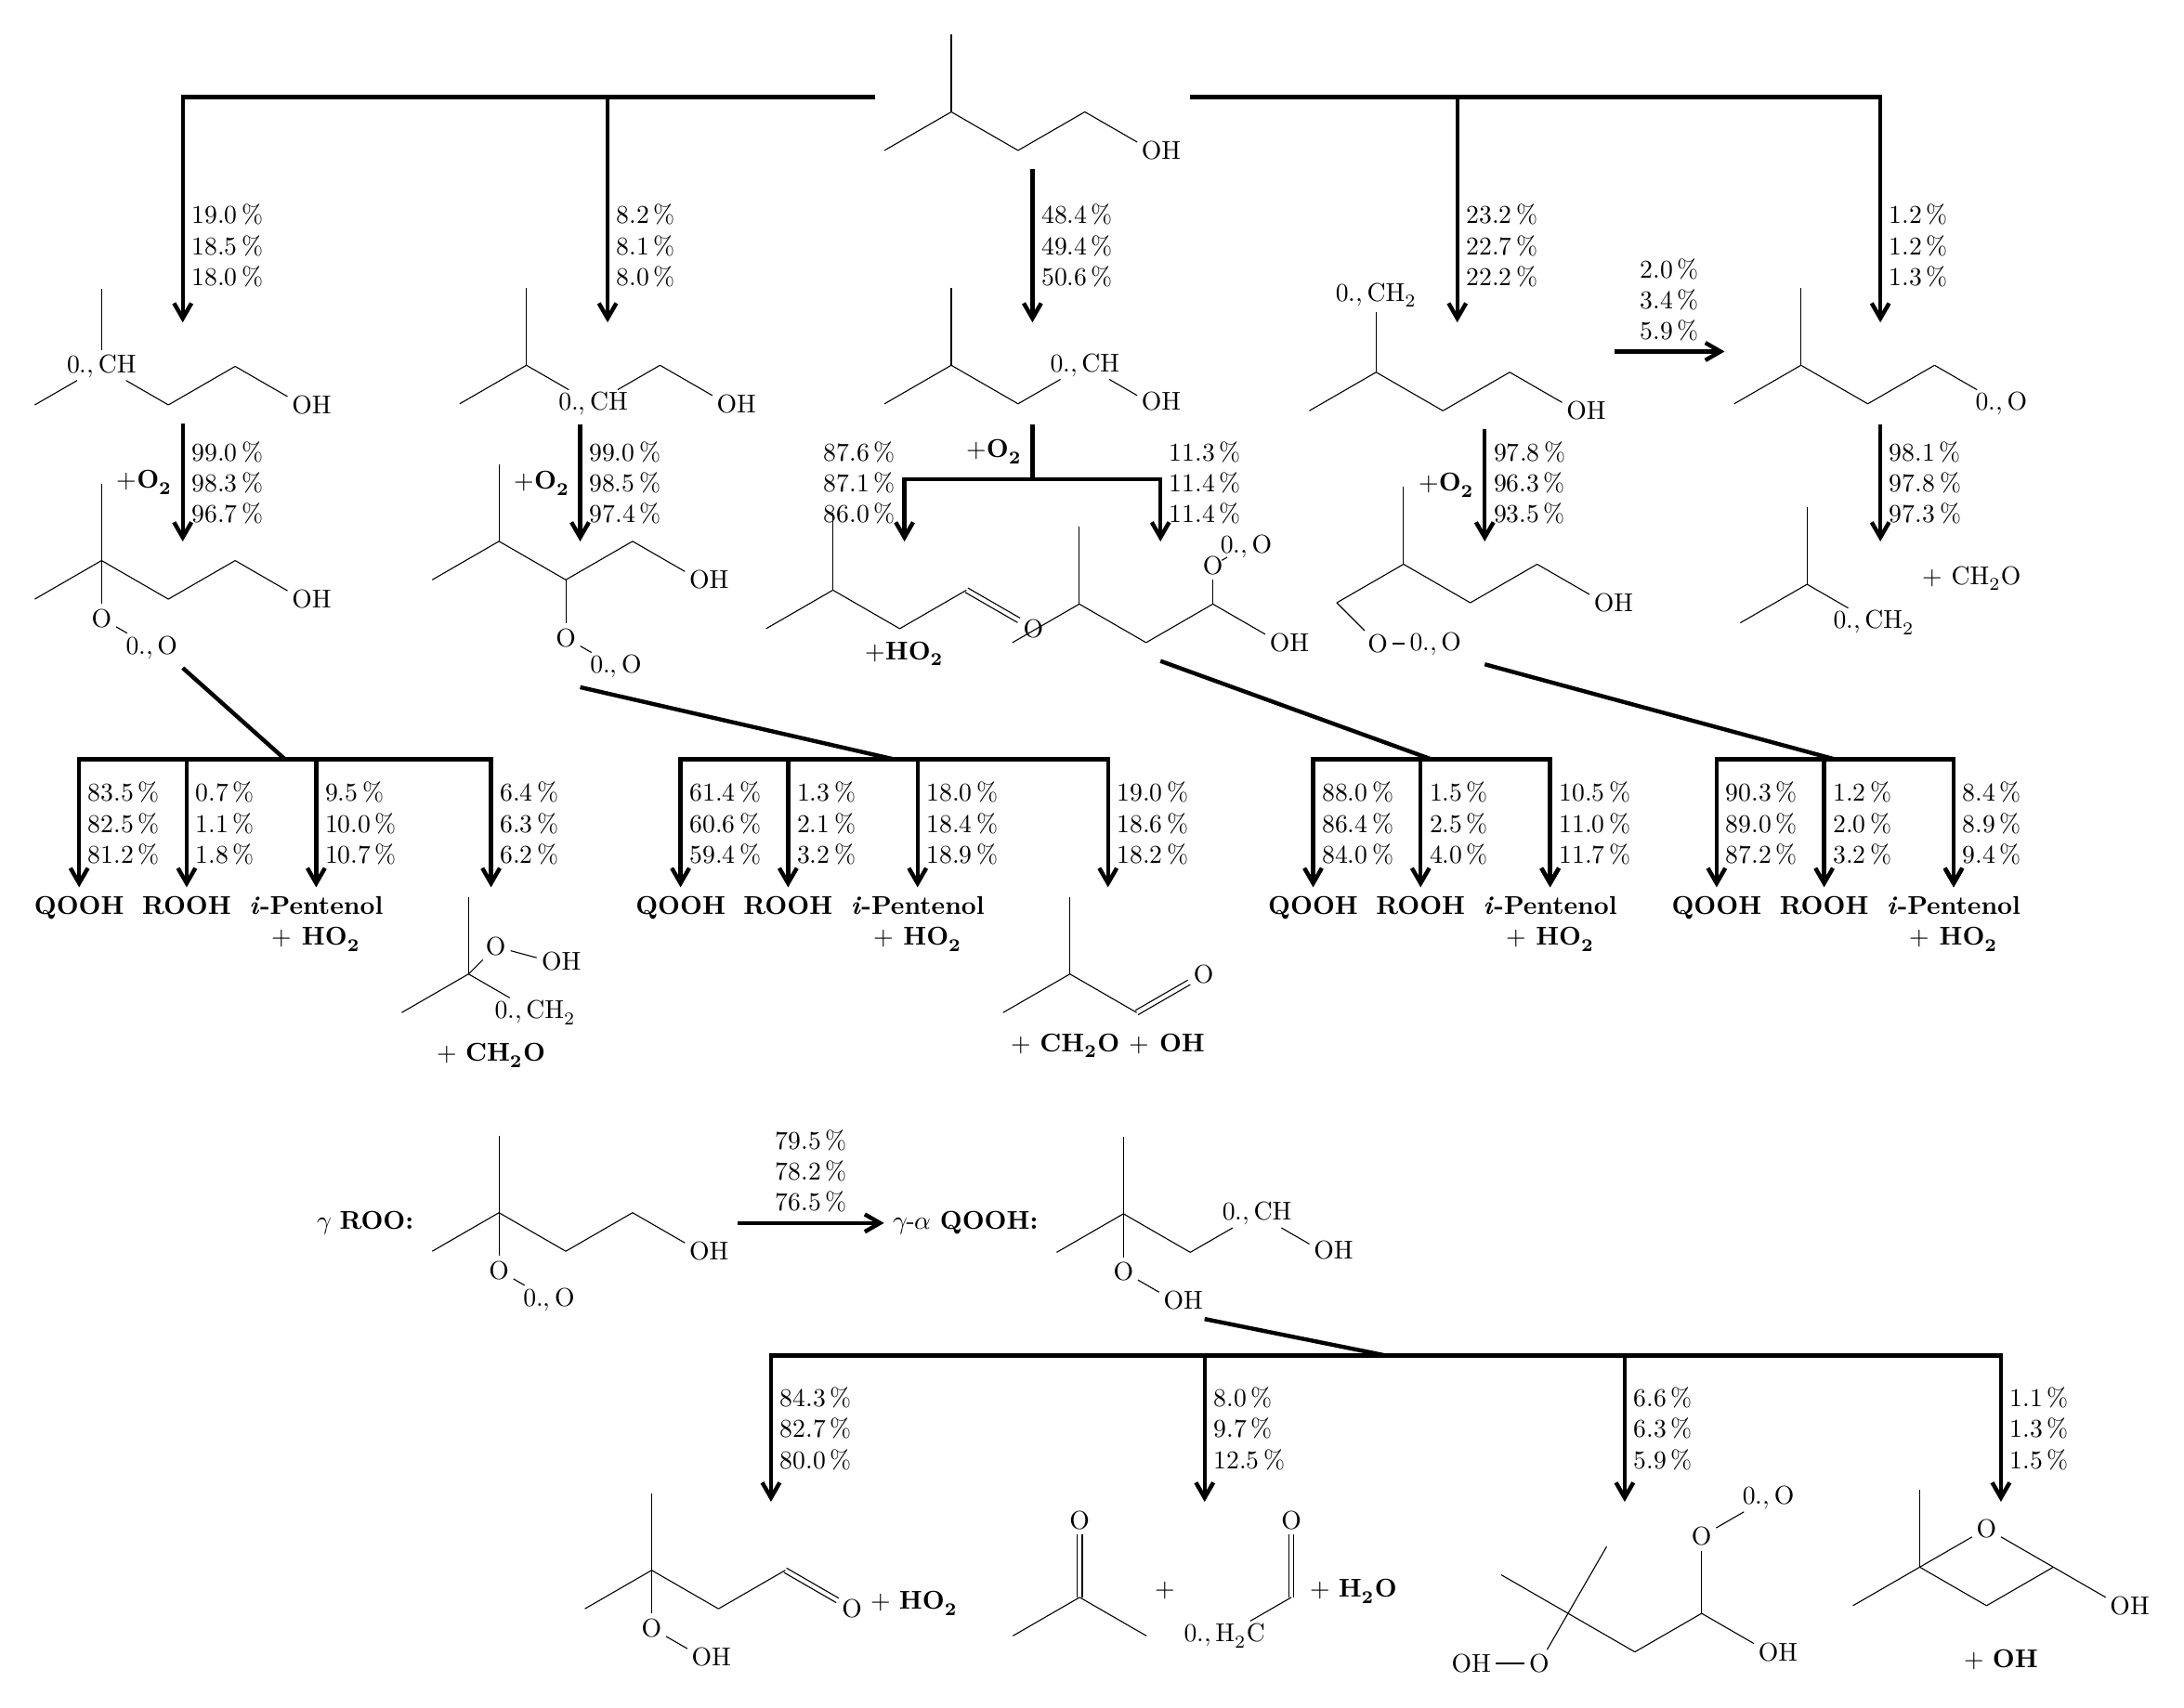
\begin{tikzpicture}[x=1cm, y=1cm]
        \begin{scope}[every node/.style={node distance=1.5}]
            \node (ipeoh) {\chemfig{-[:30]([2]-)-[:330]-[:30,,,,outer sep=10pt]-[:330]OH}};
            \node[below=of ipeoh] (aipeoh) {\chemfig{-[:30]([2]-)-[:330]-[:30]\lewis{0.,CH}-[:330]OH}};
            \node[left=of aipeoh] (bipeoh) {\chemfig{-[:30]([2]-)-[:330]\lewis{0.,CH}-[:30]-[:330]OH}};
            \node[left=of bipeoh] (gipeoh) {\chemfig{-[:30]\lewis{0.,CH}([2]-)-[:330]-[:30]-[:330]OH}};
            \node[right=of aipeoh] (dipeoh) {\chemfig{-[:30]([2]-\lewis{0.,CH_2})-[:330]-[:30]-[:330]OH}};
            \node[right=of dipeoh] (oipeoh) {\chemfig{-[:30]([2]-)-[:330]-[:30]-[:330]\lewis{0.,O}}};
        \end{scope}

        \begin{scope}[every node/.style={node distance=3 and 0.375}, on grid]
            \node[below=of gipeoh] (gipeohoo) {\chemfig{-[:30]([6,0.75]-O-[:330,0.75]\lewis{0.,O})([2]-)-[:330]-[:30]-[:330]OH}};
            \node[below left=of bipeoh] (bipeohoo) {\chemfig{-[:30]([2]-)-[:330]([6,0.75]-O-[:330,0.75]\lewis{0.,O})-[:30]-[:330]OH}};
            \node[below left=3.25 and 1.75 of aipeoh, align=center] (ipeald) {\chemfig{-[:30]([2]-)-[:330]-[:30]=[:330]O}\\$+$\textbf{\ce{HO2}}};
            \node[below right=3.25 and 1.75 of aipeoh] (aipeohoo) {\chemfig{-[:30]([2]-)-[:330]-[:30]([2,0.5]-O-[:30,0.5]\lewis{0.,O})-[:330]OH}};
            \node[below right=of dipeoh] (dipeohoo) {\chemfig{([7,0.75]-O-[0,0.75]\lewis{0.,O})-[:30]([2]-)-[:330]-[:30]-[:330]OH}};
            \node[below=of oipeoh] (oscission) {\chemfig[baseline=(c.south)]{-[:30]@{c}([2]-)-[:330]\lewis{0.,CH_2}} $+$ \ce{CH2O}};
        \end{scope}

        \begin{scope}[every node/.style={node distance=0 and 0}]
            \node[below left=3 and 0 of gipeohoo, anchor=north west] (gQOOH) {\textbf{\ce{QOOH}}};
            \node[above right=of gQOOH, anchor=north west] (gROOH) {\textbf{\ce{ROOH}}};
            \node[above right=of gROOH, align=center, anchor=north west] (giPe) {\textbf{\iPeOH}\\\textbf{$+$ \ce{HO2}}};
            \node[above right=of giPe, anchor=north west] (gscission) {\chemfig{-[:30]([2]-)(-[1,0.5]O-[:345,0.75]OH)-[:330]\lewis{0.,CH_2}}};
            \node[below=of gscission, anchor=north] {$+$ \textbf{\ce{CH2O}}};

            \node[above right=0 and 0.5 of gscission, anchor=north west] (bQOOH) {\textbf{\ce{QOOH}}};
            \node[above right=of bQOOH, anchor=north west] (bROOH) {\textbf{\ce{ROOH}}};
            \node[above right=of bROOH, align=center, anchor=north west] (biPe) {\textbf{\iPeOH}\\\textbf{$+$ \ce{HO2}}};
            \node[above right=of biPe, anchor=north west] (bscission) {\chemfig{-[:30]([2]-)-[:330]=[:30]O}};
            \node[below=of bscission, anchor=north] {$+$ \textbf{\ce{CH2O} $+$ \ce{OH}}};

            \node[above right=0 and 0.5 of bscission, anchor=north west] (aQOOH) {\textbf{\ce{QOOH}}};
            \node[above right=of aQOOH, anchor=north west] (aROOH) {\textbf{\ce{ROOH}}};
            \node[above right=of aROOH, align=center, anchor=north west] (aiPe) {\textbf{\iPeOH}\\\textbf{$+$ \ce{HO2}}};

            \node[above right=0 and 0.5 of aiPe, anchor=north west] (dQOOH) {\textbf{\ce{QOOH}}};
            \node[above right=of dQOOH, anchor=north west] (dROOH) {\textbf{\ce{ROOH}}};
            \node[above right=of dROOH, align=center, anchor=north west] (diPe) {\textbf{\iPeOH}\\\textbf{$+$ \ce{HO2}}};
        \end{scope}

        \begin{scope}[every node/.style={node distance=3 and 0.5}]
            \node[below=6 of bipeohoo] (gROO) {\chemfig{-[:30]([6,0.75]-O-[:330,0.75]\lewis{0.,O})([2]-)-[:330]-[:30]-[:330]OH}};
            \node[left=0 of gROO] {$\gamma$ \textbf{\ce{ROO}:}};
            \node[right=2 of gROO] (gaQOOHname) {$\gamma\text{-}\alpha$ \textbf{\ce{QOOH}:}};
            \node[right=0 of gaQOOHname] (gaQOOH) {\chemfig{-[:30]([6,0.75]-O-[:330,0.75]OH)([2]-)-[:330]-[:30]\lewis{0.,CH}-[:330]OH}};
            \node[below=2.5 of gaQOOH] (gascission) {\chemfig[baseline=(d)]{-[:30]@{d}([2]=O)-[:330]} $+$ \chemfig[baseline=(e)]{\lewis{0.,H_2C}-[:30]@{e}=[2]O} $+$ \textbf{\ce{H2O}}};
            \node[left=of gascission] (galde) {\chemfig{-[:30]([6,0.75]-O-[:330,0.75]OH)([2]-)-[:330]-[:30]=[:330]O} $+$ \textbf{\ce{HO2}}};
            \node[right=of gascission] (gaqoohoo) {\chemfig{-[:330]([:240,0.75]-O-[4,0.75]OH)([:60]-)-[:330]-[:30](-[2]O-[:30]\lewis{0.,O})-[:330]OH}};
            \node[right=of gaqoohoo, align=center] (gaether) {\chemfig{-[:30](-[2])(-[:30]O?)-[:330]-[:30]?-[:330]OH}\\[\baselineskip]$+$ \textbf{\ce{OH}}};
        \end{scope}

        \begin{scope}[every path/.style={draw, ultra thick, >={Straight Barb[angle=60:2pt 3]}}]
            \coordinate (line1end) at ($(aipeoh.north)-(0,0.6cm)$);
            \path[->] (ipeoh.south) -- (line1end) coordinate[midway] (mainflux);
            \path[->] let \p1 = (oipeoh), \p2 = (line1end) in (ipeoh.east) -| (\x1,\y2);
            \path[<-] let \p1 = (ipeoh), \p2 = (dipeoh), \p3 = (line1end) in (\x2,\y3) -- (\x2,\y1);
            \path[->] (dipeoh.east) -- (oipeoh.west) node[midway, above, align=center] {\flux{2.0}{3.4}{5.9}};
            \path[->] let \p1 = (gipeoh), \p2 = (line1end) in (ipeoh.west) -| (\x1,\y2);
            \path[<-] let \p1 = (ipeoh), \p2 = (bipeoh), \p3 = (line1end) in (\x2,\y3) -- (\x2,\y1);

            \coordinate (line2end) at ($(oscission.north)-(0,0.6cm)$);
            \path[->] let \p1 = (gipeohoo), \p2 = (line2end) in (gipeoh.south) -- (\x1,\y2) node [left, midway] {\textbf{$+$\ce{O2}}};
            \path[->] let \p1 = (bipeohoo), \p2 = (line2end) in ($(bipeoh.south)-(0.375,0)$) -- (\x1,\y2) node[left, midway] {\textbf{$+$\ce{O2}}};
            \path[->] let \p1 = (dipeohoo), \p2 = (line2end) in ($(dipeoh.south)+(0.375,0)$) -- (\x1,\y2) node[left, midway] {\textbf{$+$\ce{O2}}};
            \path[->] let \p1 = (ipeald), \p2 = (line2end) in (aipeoh.south) -- ++(0,-0.75) node[left, midway] {\textbf{$+$\ce{O2}}} -| (\x1,\y2);
            \path[->] let \p1 = (aipeohoo), \p2 = (line2end) in (aipeoh.south) ++(0,-0.75) -| (\x1,\y2);
            \path[->] (oipeoh.south) -- (line2end) coordinate[midway] (flux2);

            \coordinate (line3split) at ($(gQOOH.north)+(0,1.75)$);
            \path[<->] let \p1 = (gQOOH.north), \p2 = (line3split), \p3 = (gscission.north) in (\x1,\y1) -- (\x1,\y2) coordinate[midway] (flux3) -- (\x3,\y2) coordinate[midway] (gipeohoosplit) -- (\x3,\y3);
            \path (gipeohoo.south) -- (gipeohoosplit);
            \path[->] let \p1 = (gROOH.north), \p2 = (line3split) in (\x1,\y2) -- (\x1,\y1);
            \path[->] let \p1 = (giPe.north), \p2 = (line3split) in (\x1,\y2) -- (\x1,\y1);

            \path[<->] let \p1 = (bQOOH.north), \p2 = (line3split), \p3 = (bscission.north) in (\x1,\y1) -- (\x1,\y2) -- (\x3,\y2) coordinate[midway] (bipeohoosplit) -- (\x3,\y3);
            \path (bipeohoo.south) -- (bipeohoosplit);
            \path[->] let \p1 = (bROOH.north), \p2 = (line3split) in (\x1,\y2) -- (\x1,\y1);
            \path[->] let \p1 = (biPe.north), \p2 = (line3split) in (\x1,\y2) -- (\x1,\y1);

            \path[<->] let \p1 = (aQOOH.north), \p2 = (line3split), \p3 = (aiPe.north) in (\x1,\y1) -- (\x1,\y2) -- (\x3,\y2) coordinate[midway] (aipeohoosplit) -- (\x3,\y3);
            \path (aipeohoo.south) -- (aipeohoosplit);
            \path[->] let \p1 = (aROOH.north), \p2 = (line3split) in (\x1,\y2) -- (\x1,\y1);
            \path[->] let \p1 = (aiPe.north), \p2 = (line3split) in (\x1,\y2) -- (\x1,\y1);

            \path[<->] let \p1 = (dQOOH.north), \p2 = (line3split), \p3 = (diPe.north) in (\x1,\y1) -- (\x1,\y2) -- (\x3,\y2) coordinate[midway] (dipeohoosplit) -- (\x3,\y3);
            \path (dipeohoo.south) -- (dipeohoosplit);
            \path[->] let \p1 = (dROOH.north), \p2 = (line3split) in (\x1,\y2) -- (\x1,\y1);
            \path[->] let \p1 = (diPe.north), \p2 = (line3split) in (\x1,\y2) -- (\x1,\y1);

            \coordinate (line4end) at (gascission.north);
            \coordinate (line4split) at ($(gascission.north)+(0,2)$);
            \path[->] (gROO.east) -- (gaQOOHname.west) node[midway, above, align=center] {\flux{79.5}{78.2}{76.5}};
            \path[<->] let \p1 = (galde), \p2 = (gaether), \p3 = (line4end), \p4 = (line4split) in (\x1,\y3) -- (\x1,\y4) coordinate[midway] (flux4) -- (\x2,\y4) coordinate[midway] (gaqoohsplit) -- (\x2,\y3);
            \path[->] let \p1 = (gascission), \p2 = (line4split), \p3 = (line4end) in (\x1,\y2) -- (\x1,\y3);
            \path[->] let \p1 = (gaqoohoo), \p2 = (line4split), \p3 = (line4end) in (\x1,\y2) -- (\x1,\y3);
            \path (gaqoohsplit) -- (gaQOOH.south);
        \end{scope}

        \path let \p1 = (mainflux), \p2 = (aipeoh) in node[flux] at (\x2,\y1) {\flux{48.4}{49.4}{50.6}};
        \path let \p1 = (mainflux), \p2 = (oipeoh) in node[flux] at (\x2,\y1) {\flux{1.2}{1.2}{1.3}};
        \path let \p1 = (mainflux), \p2 = (dipeoh) in node[flux] at (\x2,\y1) {\flux{23.2}{22.7}{22.2}};
        \path let \p1 = (mainflux), \p2 = (gipeoh) in node[flux] at (\x2,\y1) {\flux{19.0}{18.5}{18.0}};
        \path let \p1 = (mainflux), \p2 = (bipeoh) in node[flux] at (\x2,\y1) {\flux{8.2}{8.1}{8.0}};

        \path let \p1 = (flux2), \p2 = (oscission) in node[flux] at (\x2,\y1) {\flux{98.1}{97.8}{97.3}};
        \path let \p1 = (flux2), \p2 = (gipeohoo) in node[flux] at (\x2,\y1) {\flux{99.0}{98.3}{96.7}};
        \path let \p1 = (flux2), \p2 = (bipeohoo) in node[flux] at (\x2,\y1) {\flux{99.0}{98.5}{97.4}};
        \path let \p1 = (flux2), \p2 = (ipeald) in node[left, align=right] at (\x2,\y1) {\flux{87.6}{87.1}{86.0}};
        \path let \p1 = (flux2), \p2 = (aipeohoo) in node[flux] at (\x2,\y1) {\flux{11.3}{11.4}{11.4}};
        \path let \p1 = (flux2), \p2 = (dipeohoo) in node[flux] at (\x2,\y1) {\flux{97.8}{96.3}{93.5}};

        \path let \p1 = (flux3), \p2 = (gQOOH) in node[flux] at (\x2,\y1) {\flux{83.5}{82.5}{81.2}};
        \path let \p1 = (flux3), \p2 = (gROOH) in node[flux] at (\x2,\y1) {\flux{0.7}{1.1}{1.8}};
        \path let \p1 = (flux3), \p2 = (giPe) in node[flux] at (\x2,\y1) {\flux{9.5}{10.0}{10.7}};
        \path let \p1 = (flux3), \p2 = (gscission) in node[flux] at (\x2,\y1) {\flux{6.4}{6.3}{6.2}};

        \path let \p1 = (flux3), \p2 = (bQOOH) in node[flux] at (\x2,\y1) {\flux{61.4}{60.6}{59.4}};
        \path let \p1 = (flux3), \p2 = (bROOH) in node[flux] at (\x2,\y1) {\flux{1.3}{2.1}{3.2}};
        \path let \p1 = (flux3), \p2 = (biPe) in node[flux] at (\x2,\y1) {\flux{18.0}{18.4}{18.9}};
        \path let \p1 = (flux3), \p2 = (bscission) in node[flux] at (\x2,\y1) {\flux{19.0}{18.6}{18.2}};

        \path let \p1 = (flux3), \p2 = (aQOOH) in node[flux] at (\x2,\y1) {\flux{88.0}{86.4}{84.0}};
        \path let \p1 = (flux3), \p2 = (aROOH) in node[flux] at (\x2,\y1) {\flux{1.5}{2.5}{4.0}};
        \path let \p1 = (flux3), \p2 = (aiPe) in node[flux] at (\x2,\y1) {\flux{10.5}{11.0}{11.7}};

        \path let \p1 = (flux3), \p2 = (dQOOH) in node[flux] at (\x2,\y1) {\flux{90.3}{89.0}{87.2}};
        \path let \p1 = (flux3), \p2 = (dROOH) in node[flux] at (\x2,\y1) {\flux{1.2}{2.0}{3.2}};
        \path let \p1 = (flux3), \p2 = (diPe) in node[flux] at (\x2,\y1) {\flux{8.4}{8.9}{9.4}};

        \path let \p1 = (flux4), \p2 = (galde) in node[flux] at (\x2,\y1) {\flux{84.3}{82.7}{80.0}};
        \path let \p1 = (flux4), \p2 = (gascission) in node[flux] at (\x2,\y1) {\flux{8.0}{9.7}{12.5}};
        \path let \p1 = (flux4), \p2 = (gaqoohoo) in node[flux] at (\x2,\y1) {\flux{6.6}{6.3}{5.9}};
        \path let \p1 = (flux4), \p2 = (gaether) in node[flux] at (\x2,\y1) {\flux{1.1}{1.3}{1.5}};
    \end{tikzpicture}
\end{document}